\chapter{Implementation}

An Android app had to be chosen to test and used to develop the initial
implementation. The app chosen was GSRemote, an app that I have
been developing as a hobby, since it is moderately complex, and I already
have a good understanding of the source code which make integration easier.
The app is a remote control for the web music service ``Grooveshark'',
so functions similarly to a normal music player app except it controls
a player running on the user's desktop or laptop.
Despite this, the library should be generic enough to easily integrate 
into any Android app.

\section{Integrating With the Application}

One of the requirements for the system was to be portable across
applications. It was also desirable to be as easy to implement
as possible by the app developer using minimal code and no
modifications to the app's assets.

There are two ways of adding dependencies to an Android project;
either using packaged \verb/.jar/ files as with any other java based
project, or by packaging the dependency as an Android Library
Project \cite{android-library}. A library project is similar to
an ordinary Android project, with the exception that it cannot
be run as a standalone application. This enables it to leverage
 the full functionality of the android
platform - it can make use of its own assets and layouts and manage
its own dependencies - while being self contained and portable
between projects. The only extra considerations that have to be
made with this approach is that all the project resources
(layouts, strings, images etc.) are merged with the main application's
resources, so they must be prefixed to avoid conflict with
the application the library is integrated into.

\subsection{User Interface}

A major challenge during the implementation was allowing the library
to display its UI before, during and after a task, while requiring
the application developer to write as little code specific to the
testing as possible.

The user interface appears in two forms. One is a full screen layout
that appears before and after a task, and also before the testing
begins, and the other a small strip that appears above the 
application interface during completion of a task.

The full screen layouts were initially shown by opening a separate
activity. This approach had some drawbacks, the main one being that
(at the time of writing) all activities must be registered in the
main app's manifest as opposed to the library project's manifest.
This creates extra integration work, and cannot be automatically
removed. \todo{Other drawbacks?}

In addition, this does not solve the issue of the in-task interface.
The approach used in the end for both problems takes advantage of
how android draws views.

\subsection{Injecting Views}

Interface elements on android are known as ``views'', since they
extend the View class, and are organised into a view hierarchy.
When an Activity is created, it also creates its view hierarchy
(by inflating a layout xml file or creating it programmatically)
and inserts it into a container provided by the current window.
At the root of the hierarchy is the decor view, which holds this
container along with other interface elements such as the action
bar. This entire hierarchy can be inspected with the HierarchyViewer
application that ships with the Android SDK, as shown in Figure
\ref{fig:view-hierarchy}.

\begin{figure}[h]
  \centering
  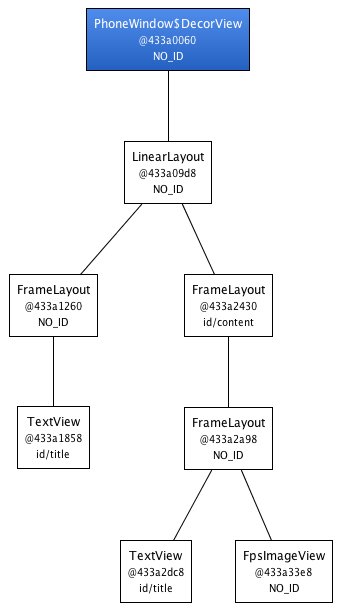
\includegraphics[width=0.35\textwidth]{images/view-hierarchy}
  \caption{The view hierarchy of a simple Android Activity. The
           view ``id/content'' is the container for the Activity's
           content. Image copied from the official Android 
           developer blog.}
  \label{fig:view-hierarchy}
\end{figure}

By obtaining a reference to the decor view using 
\verb/Activity.getWindow().getDecorView()/ the library's UI can
be either overlaid, or inserted into the top of the LinearLayout
shown beneath the DecorView in Figure \ref{fig:view-hierarchy}.

\subsection{Keeping State}

To ensure the interface remains in place as the user navigates
between activities, and does not appear on old activities, the
library must keep track of what UI (if any) is showing, and 
the current foreground Activity. When the foreground activity
pauses, due to the user navigating elsewhere or the current
activity getting destroyed (due to, for example, a screen
rotation), the extra UI must be removed from the layout and 
inserted into the new foreground activity.

With this approach, the developer need not modify any xml files
in the project, and must only include a small amount of additional
code.

\section{Integrating the Library}

The testing functionality must be easy to remove/disable if the
developer does not want it present in the released version. To know
when to begin and end tasks, inject the library's user interface
in the app, and gather data about the participant's performance,
however, some integration with the application's code is needed.
To keep this to a minimum, all interaction with the library in
performed using the static \verb/Gamify/ class. This allows for
easy removal of the library as the developer can just find all
references to this class within the main application code and remove
them. Since most Android developers use \emph{Proguard} while
compiling release versions, the rule below could be included to
automatically strip function calls to the library out of production
versions.

\begin{minted}{text}
  -assumenosideeffects class com.example.Gamify {
    <methods>;
  }
\end{minted}

Alternatively, the library can also be disabled by passing \verb|false|
when initialising. The initialisation is done by calling \verb|init|
in either the \verb|Application| or initial \verb|Activity|'s
\verb|onCreate| method, passing the two aforementioned json files.

\begin{minted}{java}
  Gamify.init(this /* Context */, true /* Enabled */,
      "challenges.json", "sequences.json");
\end{minted}

\subsection{Defining tasks}

The developer must have a way of specifying tasks and supplying
them to the library. Ideally this should be done without having
to modify any part of the library's code or assets. JSON was
chosen as the format to define tasks, since it is easy to write
and well known among developers.
The ``challenges.json'' and ``sequences.json'' files in the code
above must be included in the application's \verb+assets/+ directory.
They define the tasks that are available to perform, and what order
they will be performed in.
Each task has an id, title, description, and optional instruction
that appears at the top of the screen during a task, and defaults
to the title. The full specification can be seen in figure \ref{fig:task-spec}.
The sequences file defines groups of tasks, and which
order they will be run in. It also specifies whether to reset the
user's position in the application hierarchy after a task, or
continue from where they finished the previous task.

\begin{figure}[h]
  \begin{minted}{javascript}
  [
  
    {
      id: "Task Identifier", 
      title: "Task title",
      description: "Task description",
      instruction: "Text that appears in the in-task UI (optional)"
    }
    
  ]
  \end{minted}
  \label{fig:task-spec}
  \caption{Spec for the tasks JSON file.}
\end{figure}

\begin{figure}[h]
  \begin{minted}{javascript}
  [
  
    {
      id: "Sequence Identifier", 
      tasks: ["list", "of", "task", "ids"]
    }
    
  ]
  \end{minted}
  \label{fig:sequence-spec}
  \caption{Spec for the sequence JSON file.}
\end{figure}

\subsection{Integrating Tasks Into the Application}

To start a sequence, the developer simply calls a single method,
specifying the ID of the sequence to be started.

\begin{minted}{java}
  Gamify.startSequence("sequenceid");
\end{minted}

This will bring up the welcome screen and instructions as to how
the testing works, and allow the user to begin the first task in
the sequence. Subsequent tasks are automatically started when the
previous one is finished.

Triggering points that will complete tasks are achieved with another
method call. For example if one task was completed by playing a
song in a music app, then the corresponding code might look like
the following:

\begin{minted}{java}
  public void playSong(Song song) {
    Gamify.completeChallenge("playsong");

    //... Code to play the song
  }
\end{minted}

If the ``playsong'' task is the current task, then it will be
completed, otherwise the method call will be ignored.

Beyond this, in each \verb|Activity|'s \verb|onResume| and
\verb|onPause| methods, the library must be notified.

\begin{minted}{java}
  @Override protected void onResume() {
     super.onResume();

     Gamify.onActivityResume(this);
  }

  @Override protected void onPause() {
     super.onPause();

     Gamify.onActivityPause(this);
  }
\end{minted}

This is so user interaction can be tracked, and the library's
overlays can be shown above the foreground activity. Since good application
design encourages all activities to inherit from a single
base activity, this should not add much extra implementation overhead for the
developer. These two methods can optionally be given additional
arguments as strings, as in the case of the search activity in
Section \ref{sec:developer-feedback}.

Finally, any additional navigation points can be tracked manually,
by calling

\begin{minted}{java}
  Gamify.trackNavPoint("Navpoint name");
\end{minted}

This can be used to track fragment transactions, or anything else
the tester deems relevant.

\section{Developer Interface}

\subsection{Uploading and Storing Data}

Once a task has been completed or abandoned, the data must be
collected and centralised.

To do this, the data is converted to a JSON format and automatically
uploaded to a server running a CouchDB database. A map-reduce query
in the database is used to extract the data in the form wanted
for the graph display.

This approach was chosen for its simplicity, ease of implementation,
and the ability to iterate quickly; as CouchDB is a document oriented
database, the raw JSON data can be stored as-is without the need
to define a schema or do any preprocessing. The map-reduce is run
incrementally when new documents are received, and the results
cached, so queries remain fast.

\subsection{Accessing Data}

Another application was written to display the data gathered. It was
decided this should take the form of a web page. Since I already
had some experience with the language, coffeescript was chosen to
implement the web app, its cleaner and more expressive syntax
allowing faster development. The app queries the database and
generates the navigation graph for each task. The query returns all
the navigation paths recorded for a particular task, and the
application handles processing backtracks, merging the paths and
rendering, using the Dracula Graph library \cite{dracula-graph} to
display the final graphs.
